\chapter{Uncertainty quantification in geometry reconstruction} \label{ch:uncertainty}

\vspace{-1.5 em}
\begin{addmargin}[-0.5cm]{0cm}
  \minitoc
\end{addmargin}
\hrule
\vspace{1.5 em}

In the previous two chapters, we approached the task of geometry reconstruction using two approaches, the rather lookup table which seemed unable to scale up to molecules bigger than a triatomic molecule, and the more sophisticated optimization approach. We also ended on a troubling note, that our reconstructed geometries had unusual bond length correlations and that degenerate geometries can be rather numerous.

In this chapter we will tackle the important task of quantifying the uncertainty on our geometry reconstructions, which surprisingly has not been done by any previous study. While seemingly unrelated, it will provide us with some resolution to the unusual bond length correlations we observed.

\section{Uncertainty on a reconstructed geometry}
We will start with a rather heuristic approach to uncertainty quantification in this section. A rigorous and more sophisticated approach relying on the framework of Bayesian inference is sketched out in section \ref{sec:uncertaintyBayesian}, and other methods of uncertainty quantification are also suggested and discussed.

The question we are interested in answering is how does some amount of uncertainty on the measured momentum vectors affect the amount of uncertainty on the reconstructed geometry? We already calculated the uncertainty on the momentum vectors in section \ref{ssec:measurementUncertainty} but we cannot derive an analytic formula for the uncertainty on the molecular parameters or the atomic positions.

\subsection{A heuristic approach}
We will take a very basic approach here by generalizing a common notion in one-dimensional error analysis. If a particular measurement $\bar{x}$ of a variable $x$ carries some uncertainty $\epsilon$ such that the true value of $\bar{x}$ lies within some interval $\bar{x} - \epsilon \le \bar{x} \le \bar{x} + \epsilon$ then the true value of some arbitrary monotonic scalar function $f(x)$ that is dependent on the value of measurement will lie within some interval
\begin{equation}
  f(\bar{x} - \epsilon) \le f(\bar{x}) \le f(\bar{x} + \epsilon)
\end{equation}

If we relax the condition that $f$ be a monotonic function, then as the true value of $f(\bar{x})$ can take on any value that $f$ attains within the interval $\bar{x} - \epsilon \le \bar{x} \le \bar{x} + \epsilon$, we can say very generally that it lies between
\begin{equation}
  \min_{\displaystyle \bar{x} - \epsilon \le x \le \bar{x} + \epsilon} \; f(x)
  \le f(\bar{x})
  \le \max_{\displaystyle \bar{x} - \epsilon \le x \le \bar{x} + \epsilon} \; f(x)
\end{equation}
which may not yield a useful interval especially in the presence of discontinuities or divergences. However, for finite-valued and well-behaved functions, it may provide some overestimate of the amount of uncertainty in $f(\bar{x})$. This could be particularly accurate for small neighbourhoods about $\bar{x}$ and for slowly-varying functions $f$. As geometry reconstruction produces reasonable values for the molecular parameters, we will use this idea to quantify the uncertainty on a geometry's reconstruction.

Before Generalizing this idea to form a higher-dimensional analogue, both in the number of variables $x_i$ and the dimensionality of the function $f(\mathbf{x})$ it will be helpful to look at this idea for the case of measurement of a vector of two variables $\bar{\mathbf{x}} = (\bar{x}_1, \bar{x}_2)$ with an uncertainty described by the vector $\bm{\epsilon} = (\epsilon_1, \epsilon_2)$ and error propagation through a vector-valued function of two variables $\mathbf{f}(\mathbf{x}) = (f_1, f_2)$. We will treat the vector-valued function as non-parametrix or as a ``black box'' as the function mapping momentum measurements to geometries cannot be parameterized or given in any analytical form. In this case the true value of $\bar{\mathbf{x}}$ lies within a box described by $\bar{x}_1 - \epsilon_1 \le \bar{x}_1 \le \bar{x}_1 + \epsilon_1$ and $\bar{x}_2 - \epsilon_2 \le \bar{x}_2 \le \bar{x}_2 + \epsilon_2$. If both $f_1$ and $f_2$ both depended monotonically on the values of $x_1$ and $x_2$ then determining the range of possible values of $\mathbf{f}(\bar{x})$ would be simple. Evaluating $\mathbf{f}(x)$ for $\mathbf{x} \in \mathbf{x}_\mathrm{ep} = \lbrace (\bar{x}_1 \pm \epsilon_1, \bar{x}_2 \pm \epsilon_2) \rbrace$, where $\mathbf{x}_\mathrm{ep}$ denotes the set of $x$ endpoints, would produce $4$ point in the $f_1f_2$ plane, whose set we denote by $\mathbf{f}_\mathrm{ep}$ whose rectangular boundary encloses the possible values of $f(\bar{x})$. Of course, if $f_1$ and $f_2$ do not depend monotonically on the values of $x_1$ and $x_2$, then values of $x_1$, $x_2$ between the endpoints may produce values of $f_1$,$f_2$ that lie outside the rectangular boundary. A further heuristic would be to not only look at the endpoints, but also a set of uniformally distributed points in the $x_1x_2$ plane. This map a rectangle from the $x_1x_2$ plane to some arbitrary region in the $f_1f_2$ plane and would produce a larger number of points, whose boundary is likely to not be rectangular anymore. In the case of a more complicated boundary, then the boundary may be described by the set of convex combinations of the points in $\mathbf{f}_\mathrm{ep}$,
\begin{equation}
  \displaystyle
  \left\lbrace\left.
  \sum_{\mathbf{f} \in \mathbf{f_i}_\mathrm{ep}}^{|\mathbf{f}_\mathrm{ep}|}
  \alpha_i\mathbf{f_i}
  \right| \alpha_i \ge 0 \; \mathrm{and} \;
  \sum_i^{|\mathbf{f}_\mathrm{ep}|} \alpha_i = 1
  \right\rbrace
\end{equation}
which is the convex hull of the set of points contained in $\mathbf{f}_\mathrm{ep}$, discussed further in the next subsection.

Extending this idea to our problem of geometry reconstruction, we have $9$ measurements $\bar{\mathbf{p}} = (\bar{p}_1, \dots, \bar{p}_9)$ with uncertainty $\bm{\epsilon} = (\epsilon_1, \dots, \epsilon_9)$ and we are interested in the range of possible geometries as produced by $\mathbf{g}(\mathbf{p}) = (r_{12}, r_{23}, \theta)$. The possible values of the momentum components are contained within a $9$-dimensional hyperrectangle or box in momentum space, and we would like to obtain a $3$-dimensional region in phase space describing the set of possible geometries the measurement could correspond to. Generating a set of $N$ uniformally distributed points within the $9$-dimensional box would produce $N^9$ sets of momentum vectors, each of which we would have to reconstruct. Thus we will start by looking at the set of endpoints only, which contains $512$ ($2^9$) sets of momentum vectors. Then attempting to reconstruct a geometry for each set of momentum vectors will ideally provide us with $512$ geometries that together give us some idea into the range of possible geometries the measurement could possibly belong to. By only reconstructing the endpoints of our box in momentum space, we may be underestimating the range of possible geometries.

% % r_CO=131.677 pm, r_CS=187.161 pm, theta=169.42 deg
To carry out this idea for geometry reconstruction, we chose a representative geometry, $(r_\mathrm{CO}, r_\mathrm{CS}, \theta) = (\SI{130}{\pico\m}, \SI{190}{\pico\m}, \SI{169}{\degree})$ that does not lie in any of the degenerate regions discussed in figure \ref{fig:OCS222DegeneracyMaps} to avoid having to account for degenerate eometries. We placed an uncertainty of $5\%$ on each momentum component such that $\bm{\epsilon} = 0.05\mathbf{p}$, producing $512$ sets of momentum vectors corresponding to the corners of the $9$-dimensional box in momentum space. Reconstructing a geometry for each set of momentum vectors, we obtain $512$ geometries. The bond length and bond angle distributions are plotted as well as the bivariate relationships between the three parameters are plotted in figure \ref{fig:OCS222Uncertainty}. All $512$ sets of momentum vectors were successfully mapped to a unique geometry.

\begin{figure}
  \centering
  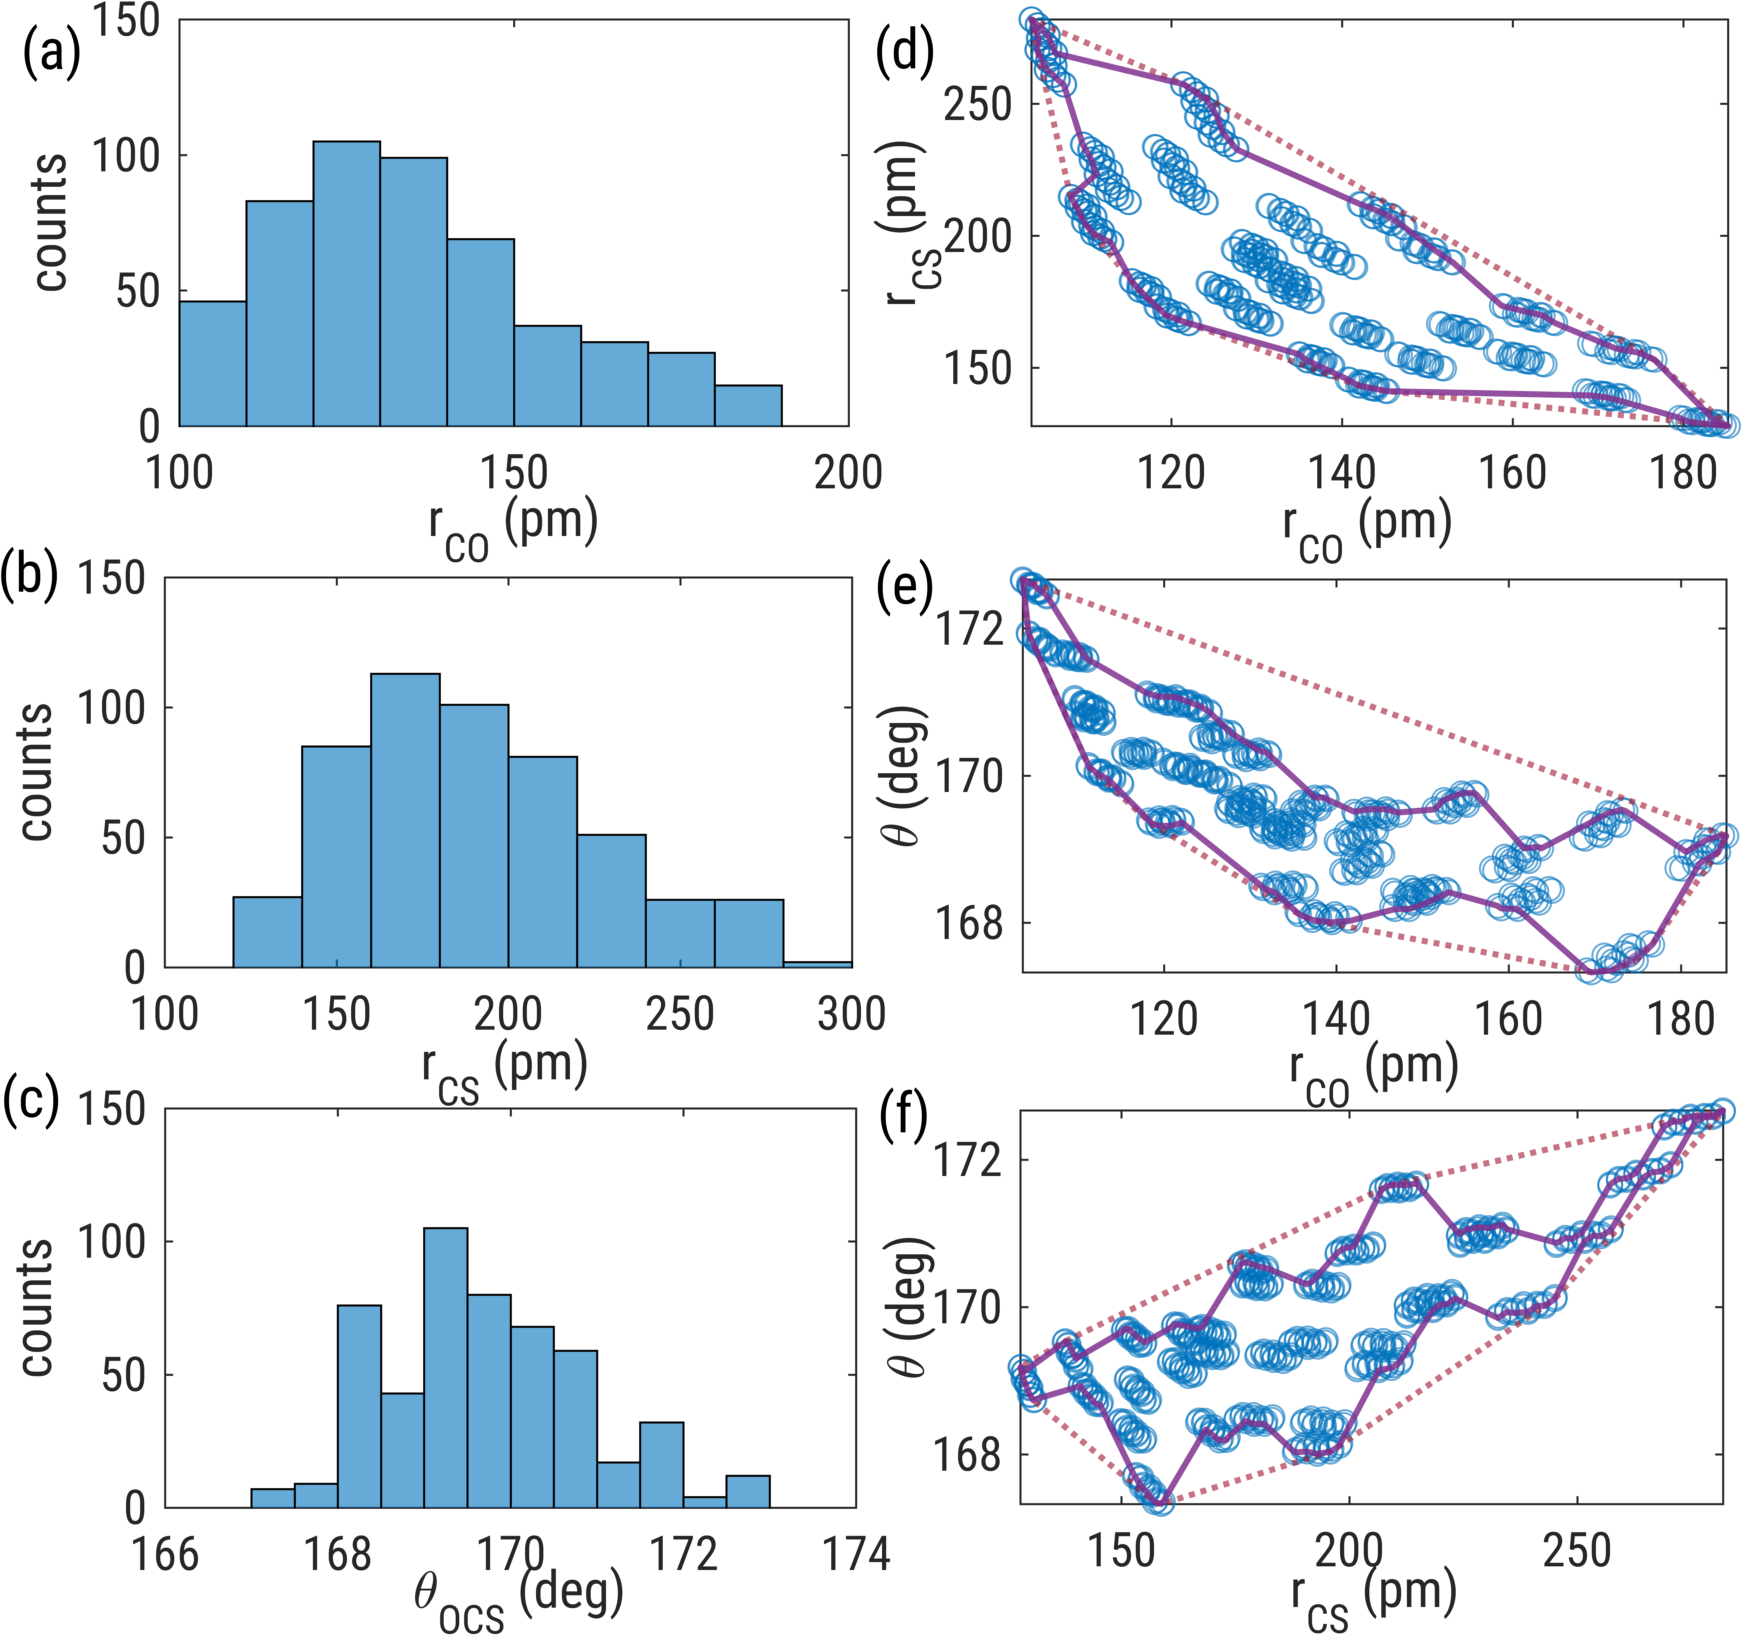
\includegraphics[width=\textwidth]{Plots/OCS222Exploration1_5percent}
  \caption[K lol.]
  {Each reconstructed geometry is plotted as an open blue circle. The boundary of the set of reconstructed geometries is calculated using two methods. The dotted red line denotes the convex hull and the solid purple line, the alpha shape of the set of points.}
  \label{fig:OCS222Uncertainty}
\end{figure}

We immediately see that we a strikingly wide range of geometries are reconstructed. Inspection suggests that the bond length and bond angle distributions roughly form a Gaussian distribution about the parameters of the geometry reconstructed without introducing any uncertainty. The distributions encompass a wide range of possible bond lengths, \SI{80}{\pico\m} for the \ch{C-O} bond and \SI{175}{\pico\m} for the \ch{C-S} bond. The variability in the bond angle is not as extreme, encompassing a \SI{6}{\degree} range of possible bond angles. It is quite shocking that a small uncertainty of only $5\%$ could correspond to such a large variety of reconstructed geometries.

The bivariate relationships are interesting and look vaugely familiar.

We will use the area formed by the set of points as a quantitative measure of uncertainty. The red dotted lines indicate the convex hull of the points while the purple solid lines indicate the alpha shape of the points. We will further discuss these concepts in the next subsection.

The bond length correlation seems to follow a reciprocal relationship, a strikingly similar one to the unusual one observed in the reconstructions of experimental data. This suggests that the unusual relationship we observed earlier may have simply been an artifact of having a finite amount of uncertainty in the momentum vectors.

Another interesting observation from the scatter plots is the clustering of geometries in phase space. Each geometry is actually extremely close to one other so that $256$ points are visible unless the scatter plots are very closely inspected, suggesting some sort of splitting. As we picked one of two extreme values for each momentum component, each component may be responsible for one of these splittings. This suggests that some uncertainty in certain momentum components may have a much greater effect on the uncertainty of reconstructed geometries. We will investigate this effect in the next section.

\subsection{Convex hulls and alpha shapes}
To quantify the uncertainty in the geometries, we will use two useful concepts from computational geometry, namely convex hulls and alpha shapes, which allow us to assign a shape and a volume to a set of points, and thus provide an additional hueristic quantitative measure of uncertainty.

The convex hull of a set of points $S$ is the set of all convex combinations of its points. An analogy would be to stretch a rubber band around the set of points and let it rest, its final shape being the convex hull.

Many algorithms exist to calculate the convex hull of a set of points, especially in 2 or 3 dimensions.

The concept of an alpha shape is a generalization of the convex hull first introduced by \citet{Edelsbrunner83} for two-dimensional shapes, then for three-dimensional shapes \citep{Edelsbrunner94}. Interestingly, alpha shapes have been used to analytically compute shapes for macromolecules such proteins and estimate their molecular areas and volume \citep{Liang98}. An interesting analogy of alpha shapes uses ice cream scoopers.

The nice thing about convex hulls is that they are unique for each set of points, while multiple distinct alpha shapes exist. This is a desirable property of alpha shapes as there is no formal concept of shape so no algorithm can determine the correct shape for a set of points. However, the concept allows for an $\alpha$ to be picked that produces the most desirable shape. 

While a very haphazard measure of uncertainty, they are much easier to employ than the sophisticated uncertainty quantification framework of Bayesian inference (section \ref{sec:uncertaintyBayesian}) and will come in handy when we perform some exploratory uncertainty analysis in section \ref{sec:uncertaintyAnalysis}. Our needs are rather basic at this point.

We end by providing a cool figure showcasing the three-dimensional convex hull and alpha shape in molecular phase space.

% figure Z here

\section{Determining the sources of uncertainty}
We saw in figure X that certain momentum components may have a much greater effect on the uncertainty on a reconstructed geometry, or that geometry reconstruction is much more sensitive to certain momentum components than others.

We will attempt to explore this effect and pinpoint the momentum components responsible for introducing the most and the least uncertainty. To do this for the oxygen's $p_x$ component for example, we will look at the $256$ sets of momentum vectors that represent the extreme end and plot their position in the $r_\mathrm{CO}-r_\mathrm{CS}$ plane in phase space. Doing this for each component, we should have $9$ plots in total.

% figure Y here

We definitely see that some components are more responsible than others. For example, the A component seems largely responsible for variability in $r_\mathrm{CO}$ and the B component seems responsible for variability in the $r_\mathrm{CS}$ component. Interestingly, removing the C component seems to produce a plot almost exactly like the one in figure X, suggesting that uncertainty in C introduces a negligible amount of uncertainty in the reconstructed geometries.

This result has implications for the design and operation of Coulomb explosion imaging experiments, especially if the determination of molecular structure is a concern. The CEI apparatus could be built with the aim of minimizing certain momentum components. The laser's polarization may also have an effect.

The exact dependence observed in figure Y may be due to experimental considerations. Or choice of momentum convention? Further investigation is certainly warranted.

\section{Exploratory uncertainty analysis} \label{sec:uncertaintyAnalysis}
Let's put a range of uncertainties on the momentum vectors and observe how much uncertainty we have on the reconstructed geometries. We will use the widths of the distributions and the convex hull and alpha shape areas and volumes to quantify the uncertainty with the aim of finding how uncertainty in geometry reconstruction varies as a function of uncertainty in the momentum vectors.

% Various figures here

Interestingly, we are always able to reconstruct the geometry.

\section{Uncertainty quantification using Bayesian inference} \label{sec:uncertaintyBayesian}
The heuristic uncertainty quantification performed in the previous three sections has provided some significant insights on the problem of geometry reconstruction, and emphasized the large effect that measurement uncertainty must have played in our reconstruction of experimental data. This emphasizes the importance of tackling the task of uncertainty quantification in a rigorous and sophisticated manner, in which case the Bayesian inference framework provides the answer.

% Philosophy? objective vs. subjective Bayes, frequentist vs. Bayesian, etc.
The Bayesian point of view provides a more natural and intuitive way of thinking about uncertainty in the physical sciences.

% Why Bayesian inference is perfect for inverse problems.

Bayesian statistics actually predates the much more commonly taught frequentist statistical methods but has made a strong resurgence in recent years due to rising computational abilities and more recently, available software for parameter estimation in statistical models using Markov chain Monte Carlo.

\subsection{Elementary concepts}
% Ideas?: credibility, models, parameters, distributions.
% Theory?: Bayes Theorem, prior predictive, posterior, posterior mode (read up).
% Bayes’ theorem: we just need to do a multi-dimensional integral

\subsection{Markov chain Monte Carlo}
% The basic idea
Performing the multi-dimensional integral can be very difficult. The integral is usually approximated using Markov Chain Monte Carlo.
% Markov Chain Monte Carlo: transition kernel, checking for convergence, Metropolis-Hastings algorithm, Gibbs Sampling, Hamiltonian MCMC

\subsection{Other Bayesian methods}
Uncertainty quantification for inverse problems in the Bayesian framework.

% Tikhonov regularization? Actually Bayesian inversion is a great alternative?

% MMMGRUBS alternative idea: Time evolve the system backwards from the measurement using a Kalman filter to keep track of the error in the geometry. My guess: The magnitude of the error will be much larger than the physical size of the molecule.

\section{Conclusions}